\documentclass[twocolumn]{article}
\usepackage[utf8]{inputenc}
\usepackage[T1]{fontenc}
\usepackage[margin=1in]{geometry}
\usepackage{graphicx}
\usepackage[font=small,labelfont=bf]{caption}
\setlength{\columnsep}{0.3in}
\title{Kilonovaen og oprindelsen af guld}
\author{Jonatan Selsing \\
	The Cosmic Dawn Center \\
	 Niels Bohr Instituttet  \\
	 Københavns Universitet \\
	}

\date{\today}
% Hint: \title{what ever}, \author{who care} and \date{when ever} could stand 
% before or after the \begin{document} command 
% BUT the \maketitle command MUST come AFTER the \begin{document} command! 
\begin{document}

\maketitle


\begin{abstract}
I denne her artikel vil jeg introduce et fænomen som for først for ganske nyligt er trådt frem på den astronomiske scene, nemlig kilonovaer. Kilonovaer har vist sig at være nogle af de mest eksotiske, sjældne, og samtidig betydningsfulde begivenheder, der sker i universet. En kilonova er et resultat af sammenstødet mellem to neutronstjerner, eller en neutronstjerne og et sort hul. I sammenstødet bliver neutron-stjerne materiale slynget ud i universet, og dette materiale bliver til alle de tungeste grundstoffer vi kender, som bla. guld, sølv og platin. 
\end{abstract}

\section{Introduktion}
Den 17. august 2017 skete der noget specielt i de tre tyngebølgedetektorer der udgør LIGO/Virgo samarbejdet. For første gang registrerede detektorerne det karakteristiske "tyngdebølge-skvulp" fra et binært system, hvis vægt begrænset til ca. 2.8 somasser og derfor konsistent med to neutronstjerner \cite{abbotta}. Uafhængigt, og forsinket med 1.7 s, detekterede GBM (Gamma-ray Burst Monitor) instrumentet ombord rum-teleskopet \textit{Fermi}, et kort signal af gamma-stråler, konsistent med den type signal vi kender fra korte gamma-glimt. Derfra vidste vi med det samme, at tyngdebølgesignalet rejste sammen med noget elektromagnetisk stråling, hvilket betød, at vi for første gang i verdenshistorien havde muligheden for at se det optiske modstykke til et tyngdebølgesignal. Dette optiske modstykke var på forhånd teoretiseret til at være lysstrækt nok til, at vi ville kunne se det, samt potentielt selt set være kilden til alle de tungeste grundstoffer i universet \cite{lattimer}. På grund af formodningen om betydningen af at finde dette modstykke, var det virkeligt vigtigt at sikre en hurtig opfølgning med teleskoper, inden det optiske lys blev for svagt til se mere. 

Ved at triangulere på baggrund af ankomst-tidspunktet af signalet i tyndebølgedetektorerne kunne LIGO/Virgo finde frem til, at dette her sammenstød skete over den sydlige halvkugle, inden for et område på størrelse med fuldmånen, hvilket er ca 28 kvadratgrader. Dette lyder måske ikke af meget, men en typisk størrelse et teleskop dækker omkring 0.25 kvadratgrad, så det kræver alligevel en del billeder at dække hele området. 10.9 timer efter den simultane detektion af tyngdebølger og gamma-stråler blev det optiske modstykke fundet. Detektions-billederne er vist i figur \ref{fig1}, hvor det øverste, højre billede er det første billede der blev taget af kilonovaen. Så snart det optiske modstykke blev fundet, var den positionelle usikkerhed så lille, at en verdensomspændende opfølgningskampagne kunne iværksættes, hvor teleskoper der dækker hele det elektromagnetiske spectrum kunne pege mod dette nyopdagede astronomiske fænomen.

\begin{center}
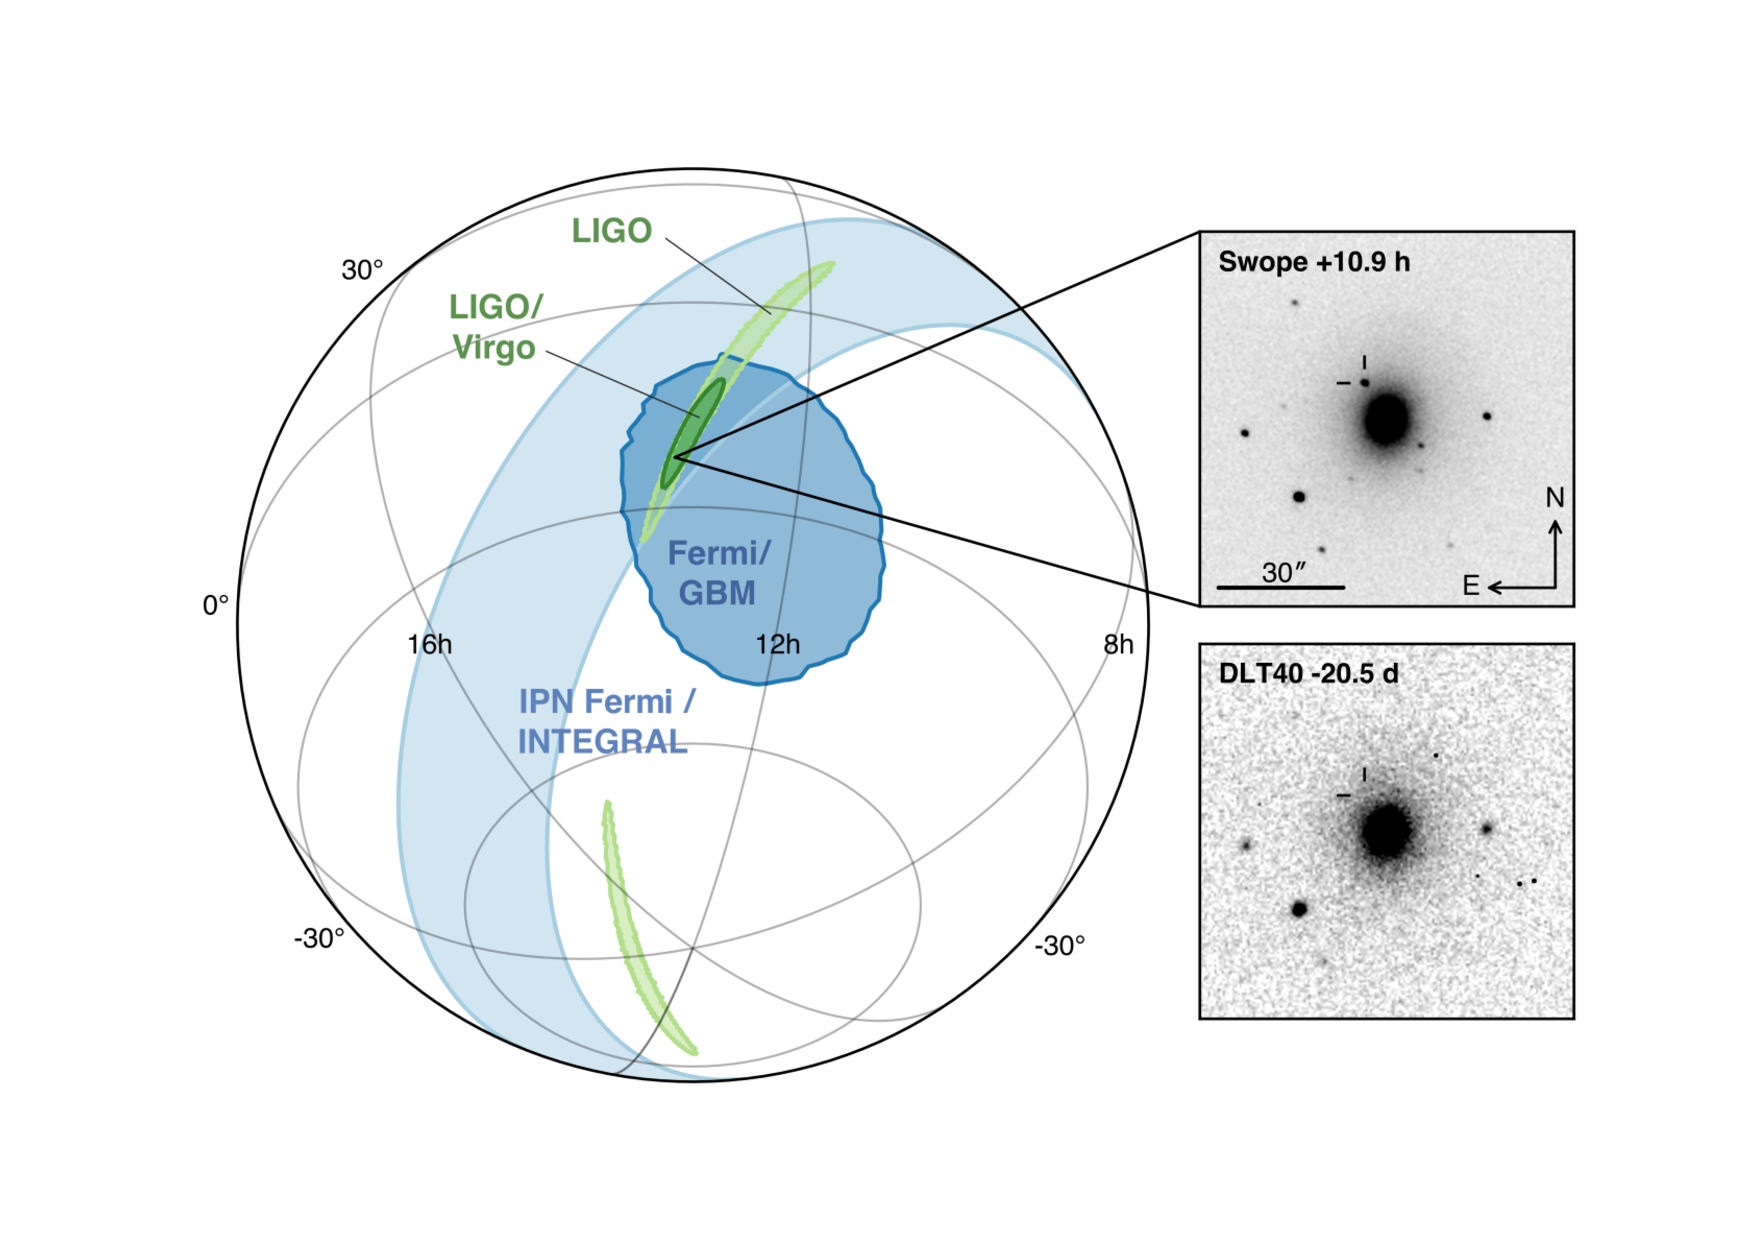
\includegraphics[width=\columnwidth]{GW170817_MMA_Skymap} \label{fig1}
\captionof{figure}{Lokaliseringen af kilonovaen baseret på ankomst-tidspunktet af tyngebølgesignet til de forskellige detektorer, samt GBM lokalisationen. Figuren er taget fra \cite{abbottb}}
\end{center}





\section{Baggrund}\label{bag}

For at forstå, hvorfor dette fænomen var søgt efter med sådan en ihærdighed, samt hvorfra navnet kilonova stammer, kræver det til baggrundsviden. 

Den kemiske sammensætning af universet, er på et hvert tidpunkt et produkt af startbetingelserne, samt hvilke processer der undervejs opererer for at drive den kemiske berigelse. I begyndelsen af vores observerbare univers var Big Bang. Big Bang efterlader et univers primært bestående af hydrogen og helium. Tyngdekraften får ur-gassen til at fragmentere i mindre og mindre stykker, som til sidst danner galakserne og deres bestanddele - stjerner. Under tilpas høj tæthed og temperatur (der bliver opnået inde i centrum af alle stjerner), undergår hydrogen og helium kerne fusion. Kernefusion er den process hvorved to atomkerner fusionerer. To hydrogen-kerner støder sammen og laver helium, tre helium-kerner støder sammen og laver karbon, en karbonkerne og en heliumkerne støder sammen og laver ilt, osv... På denne måde bliver grundstofferne tungere og tungere. Denne process kan lade sige gøre, fordi bindingsenergien af tungere grundstoffer er højere end for lettere grundstoffer. Der kan derfor vindes energi ved at omdanne lette grundstoffer til tunge. Denne fusions-process er energikilden til alle tændte stjerner i universet. 

\begin{center}
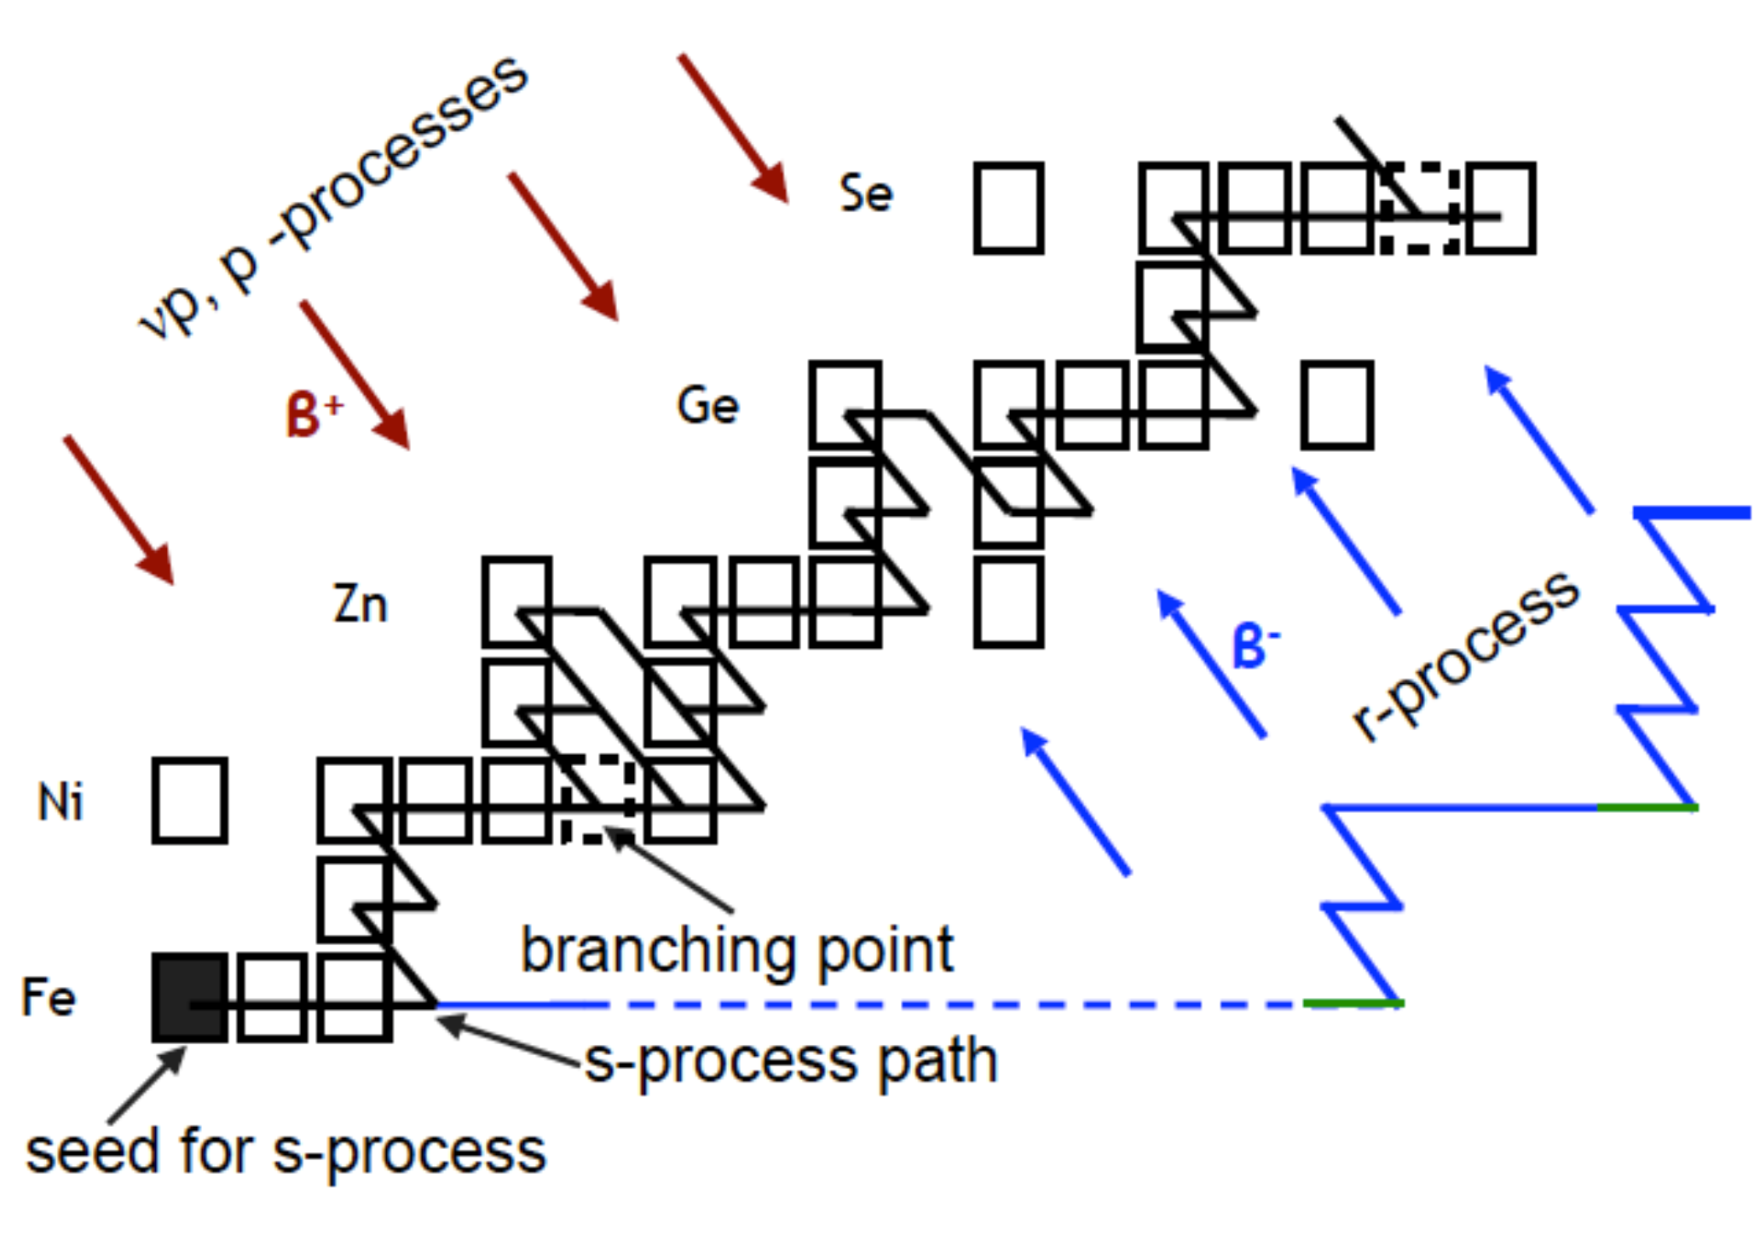
\includegraphics[width=\columnwidth]{r-process2.pdf}
\captionof{figure}{Illustration af $s$- og $r$ processen. $S$-processen er dem sorte streg der følger de stabile isotoper. Steder, hvor der er huller i isotop-stigen gør, at $s$-processen skal bruge lang tid til at kravle opad i atomtal. $R$-processen, derimod, kan meget hurtigt berige kim-grundstoffer til de tungeste grundstoffer i vores periodiske system.}
\end{center}

De højeste bindingsenergier findes i grundstofferne jern ($\mathrm{Fe}_{26}^{56}$) og nikkel ($\mathrm{Ni}_{28}^{58}$), med atomtallene hhv. 26 og 28 og massetallene hhv. 56 og 58. Atomtallet betyder at de hver indeholder hhv. 26 og 28 protroner og massetallene betyder at de hver indeholder hhv. 56 og 58 protroner og neutroner. Fordi jern og nikkel har de højeste bindingsenergier, er det også de tungeste grundstoffer der naturligt laves ved fusion. Tungere grundstoffer end jern og nikkel er alle sammen lavet på basis af neutronindfangning. Neutronindfangning betyder at en atomkerne optager en fri neutron. Dette kan ske, fordi neutronen er ladningsløs, og der ikke er nogen elektrostatisk frastødning mellem atomkernen og den frie elektron. Ved en neutronindfangning stiger massetallet for et grundstof ned 1, fordi der er kommet en ekstra neutron i kernen. F.eks, hvis en jernkerne og en fri neutron støder sammen, vil det hedde $\mathrm{Fe}_{26}^{56} + \mathrm{n} \rightarrow \mathrm{Fe}_{26}^{57} + \gamma$, hvor n er neutronen, og $\gamma$ er en foton. $\mathrm{Fe}_{26}^{57}$ er en stabil isotop af jern, men hvis nu der bliver ved at blive indfanget neutroner, vil det kunne hedde $\mathrm{Fe}_{26}^{58} + \mathrm{n} \rightarrow \mathrm{Fe}_{26}^{59} + \gamma$. $\mathrm{Fe}_{26}^{59}$ er \textit{ikke} en stabil isotop, og vil beta-henfalde til cobalt og en neutrino ( $\mathrm{Fe}_{26}^{59} \rightarrow  \mathrm{Co}_{27}^{59} + \nu_e$), hvorved atomtallet stiger med 1. Beta-henfaldet er den process hvorved en neutron henfalder til en protron, og kan skrives $n \rightarrow p + e^- + \nu_e$. 

\begin{center}
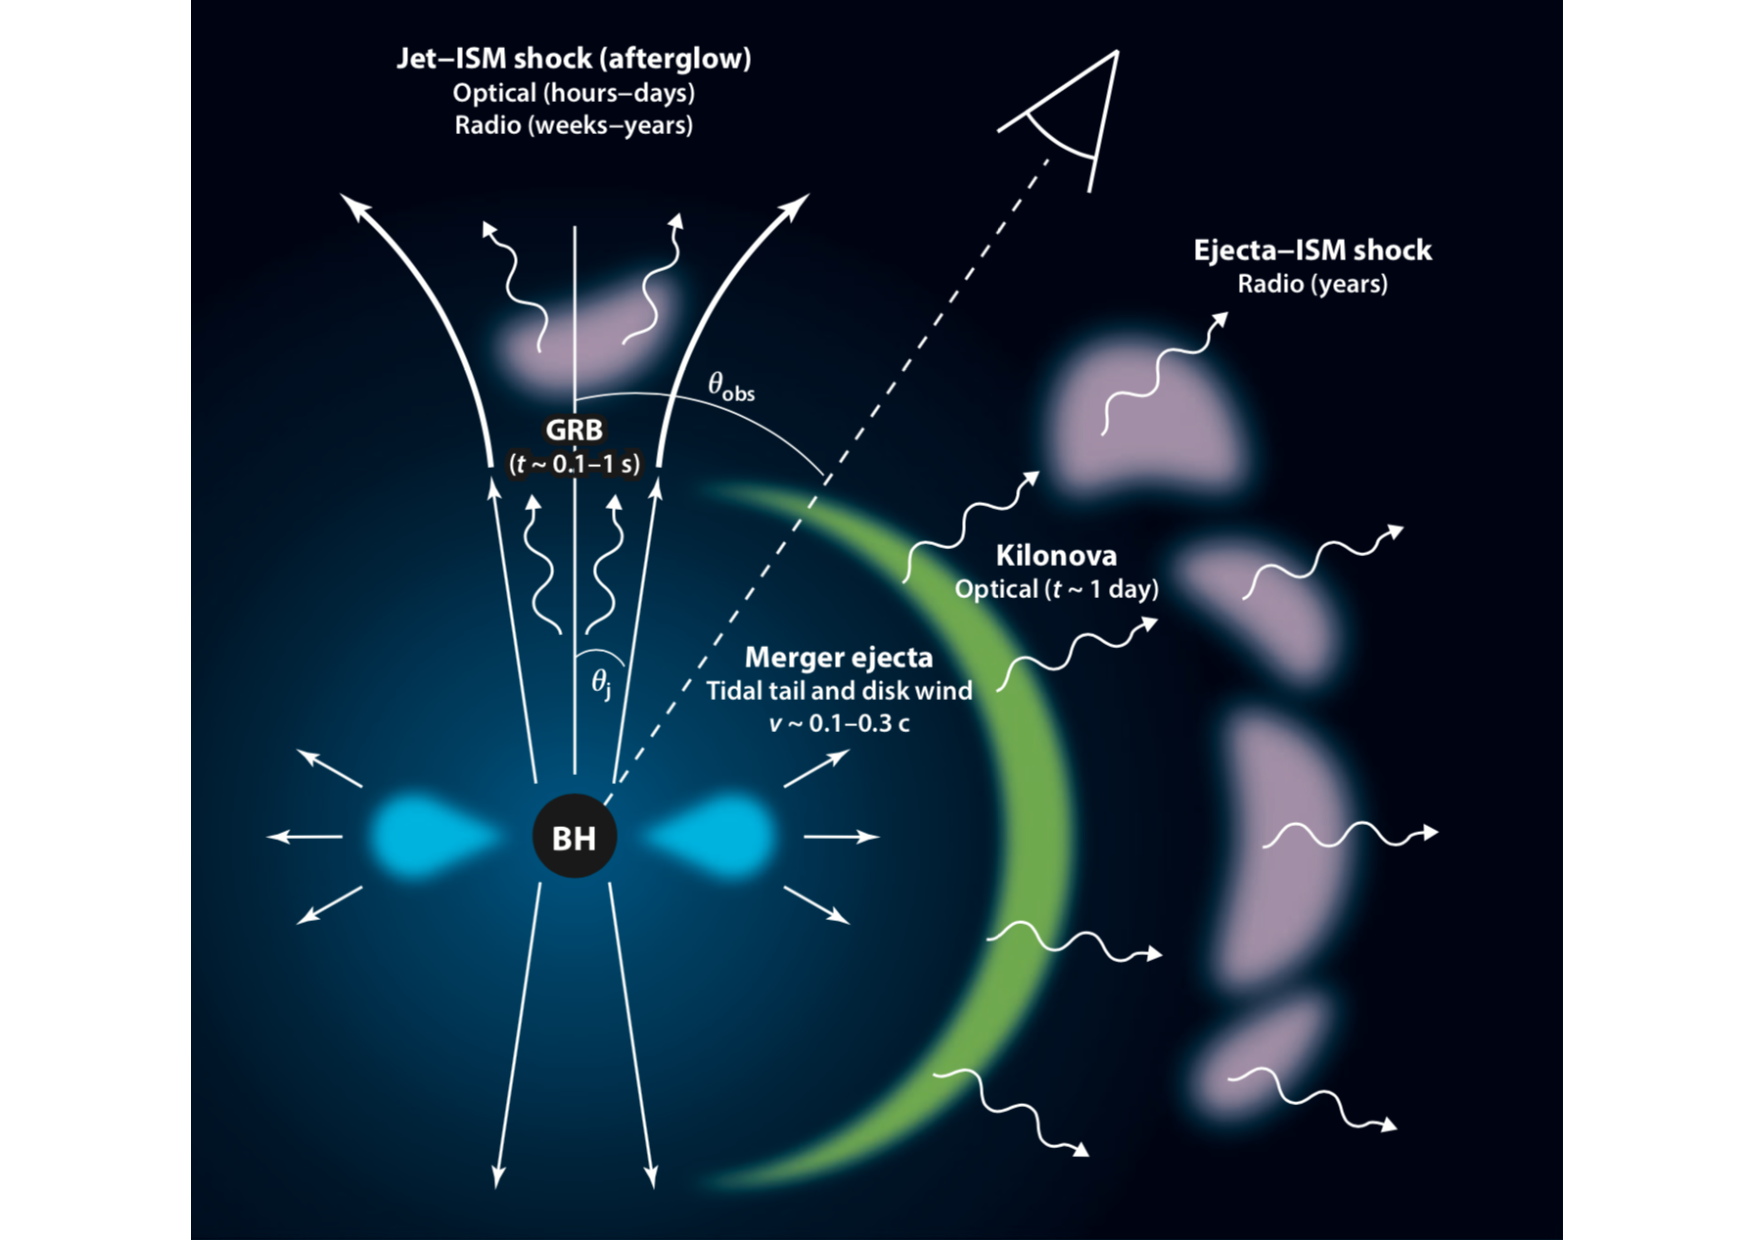
\includegraphics[width=\columnwidth]{KN_scematic_berger.pdf}
\captionof{figure}{Skematisk oversigt over, hvordan vi forestiller os kilonovaen bliver dannet. Centralt er det nydannede sorte hul (BH), hvor de to blå "dråber" representerer de to neutron stjerner der er ved at smelte sammen. Figuren er  fra \cite{berger}}
\end{center}

\section{$r$-processen}\label{rproc}


Neutronindfangningsprocessen opdeles i to klasser, som bliver sepereret på baggrund af neutronindfangningsraten - altså hastigheden hvormed neutroner bliver fanget - i forhold et beta-henfaldsraten. s-processen, hvor s står for slow, betyder neutronindfangningsraten er langsommere end beta-henfaldet. I s-processen vil enhver neutronindfangning til en ustabil isotop være efterfulgt at et beta-henfald til et grundstof med én mere protron, og derfor højere i det periodiske system. S-processen kan i princippet give alle de tungere grundstoffer op til polonium ($\mathrm{Po}_{210}^{84}$), men er for langsom til at kunne berige vores univers i tilstrækkelig grad, hurtigt nok. r-processen (r står for rapid), derimod, er den hurtige process, hvor neutroner bliver indfanget hurtigere end det nye element kan nå at beta-henfalde. Denne process kan operere på meget korte tidsskalaer, og har i princippet ikke nogen øvre grænse for, hvor tunge grundstoffer det kan lave. Problemet med $r$-processen er at, den kræver en enorm tæthed af frie neutroner - en tæthed der i praksis er meget svær at opnå. Der er dog ét sted i universet, hvor neutrontætheden er enorm. Neutronstjerner. Neutronstjerner er restproduktet af en stor del af de supernovaer, der har hydrogen i deres spektre (type II), og er kompakte objekter der ikke er større end ca. 10 km i diameter. Neutronstjerner vejer som regel omkring 1.4 gange så meget som vores sol, og består sandsynligvis i høj grad af neutroner, med en tynd ydre skal af jern. Grunden til dette, er at tyngdekraften er så høj, at de elektroner og protroner der måtte være, er blivet presset sammen til neutroner. Hvis man på én eller anden måde kan få en neutronstjerne revet fra hinanden, ville det kunne give den tilstrækkelige tæthed af frie neutroner til at drive $r$-processen.

\section{Neutronstjernesammenstød}\label{ns}


I 1974 blev det første binære neutronstjernesystem fundet, kaldet Hulse-Taylor systemet, efter dets opdagere. Her fandt man det første bevis for tilstedeværelsen af tyngdestråling, fra henfaldet af omløbsbanen af dette system. (Mellem omdragelsen af kilonovaen og offentliggørelsen, blev Rainer Weiss, Barry C. Barish og Kip S. Thorne tildelt Nobelprisen i fysik for opdagelsen af tyngdebølger.) Henfaldet af omløbsbanen af de to neutronstjerner betyder, at de langsomt bevæger sig nærmere og nærmere hinanden under udsendelse af tyngdebølger, i overensstemmelse med Einsteins generelle relativitetsteori. De to neutronstjerner i Hulse-Taylor systemet vil støde sammen om ca. 300 millioner år.  

Sammenstødet mellem to neutronstjerner har, fordi det er det optimale sted for $r$-processen, været fokus for en del teoretiske undersøgelser. De modelleder der er udviklet for sammenstødet er enige om at ved et sammenstød ved en væsentlig del af den totale masse blive slynget ud i rummet, i det plan som neutronstjerner roterer om hinanden. Grunden til dette, er at som omløbsbanen henfalder, vil rotationshastigheden af systemet stige. På et tidpunkt, ca sammetidig som de to neutronstjerner støder sammen, vil rotationshastigheden af de yderste dele af neutronstjernerne være hurtigere end undvigelseshastigheden for en binært neutronstjerne system, og derfor vil de blive slynget ud. Den store mængde, nu frie, neutroner vil med det samme blive absorberet af jern-laget og drive $r$-processen hele vejen til de tungeste grundstoffer. De nydannede, meget tunge grundstoffer, vil så beta-henfalde og radioaktict spalte under udsendelse af en meget stor mænge lys. De teoretiske modeller forudsiger, at den totale mængde lys der bliver udsendt, vil være ca. 1000 gange så stor, som den mængde lys der bliver udsendt ved en normal nova. Kilo nova. Tusind gange så lysstærk som en nova. Alternativt bliver det optiske modstykke til sammenstødet også kaldt macronova. 

Neutronsternesammenstød har yderlige to fysiske signaturer, som var yderst eftersøgte. Hidtil havde man ikke nogle troværdige målinger, af hvilke systemer der giver anledning til korte gammaglimt. Ved den samtidige detektion at et kort gammaglimt, tyngedebølger fra binært system, der vejer ca. ligeså meget som to neutronstjerner, og en kilonova, var der endegyldigt bevis for, at i hvert fald nogle korte gammaglimt bliver lavet af neutronstjernesammenstød. Den anden signatur, er den at "lydstyrken" af tyngdebølger er bestemt af perioden af bølgen. Fra rødforskydningen af værtsgalaksen og denne periode, kan vi ret præcist måle en absolut afstand - en måling der er meget svær at lave, og som har stor betydning for vores estimat af universets alder og udvidelseshistorie. Denne måling er konsistent med målinger fra f.eks PLANCK teleskopet. Ved at måle flere af disse afstande håber vi på at kunne finde afvigelser mellem PLANCK målingerne og tyngdebølgerne, vil vil åbne døren til nye modeller for vores univers. 


\section{Observationerne}\label{obs}

Fordi neutronstjernesammenstødet var forbundet med stor forventning, var det højt priorteret på teleskoper verden over. Derfor findes der et væld af observationer fra Røntgenstråling til radio, som i store træk bekræfter de teoretiske forestillinger om hvordan sådan et fænomen måtte se ud. 


\begin{center}
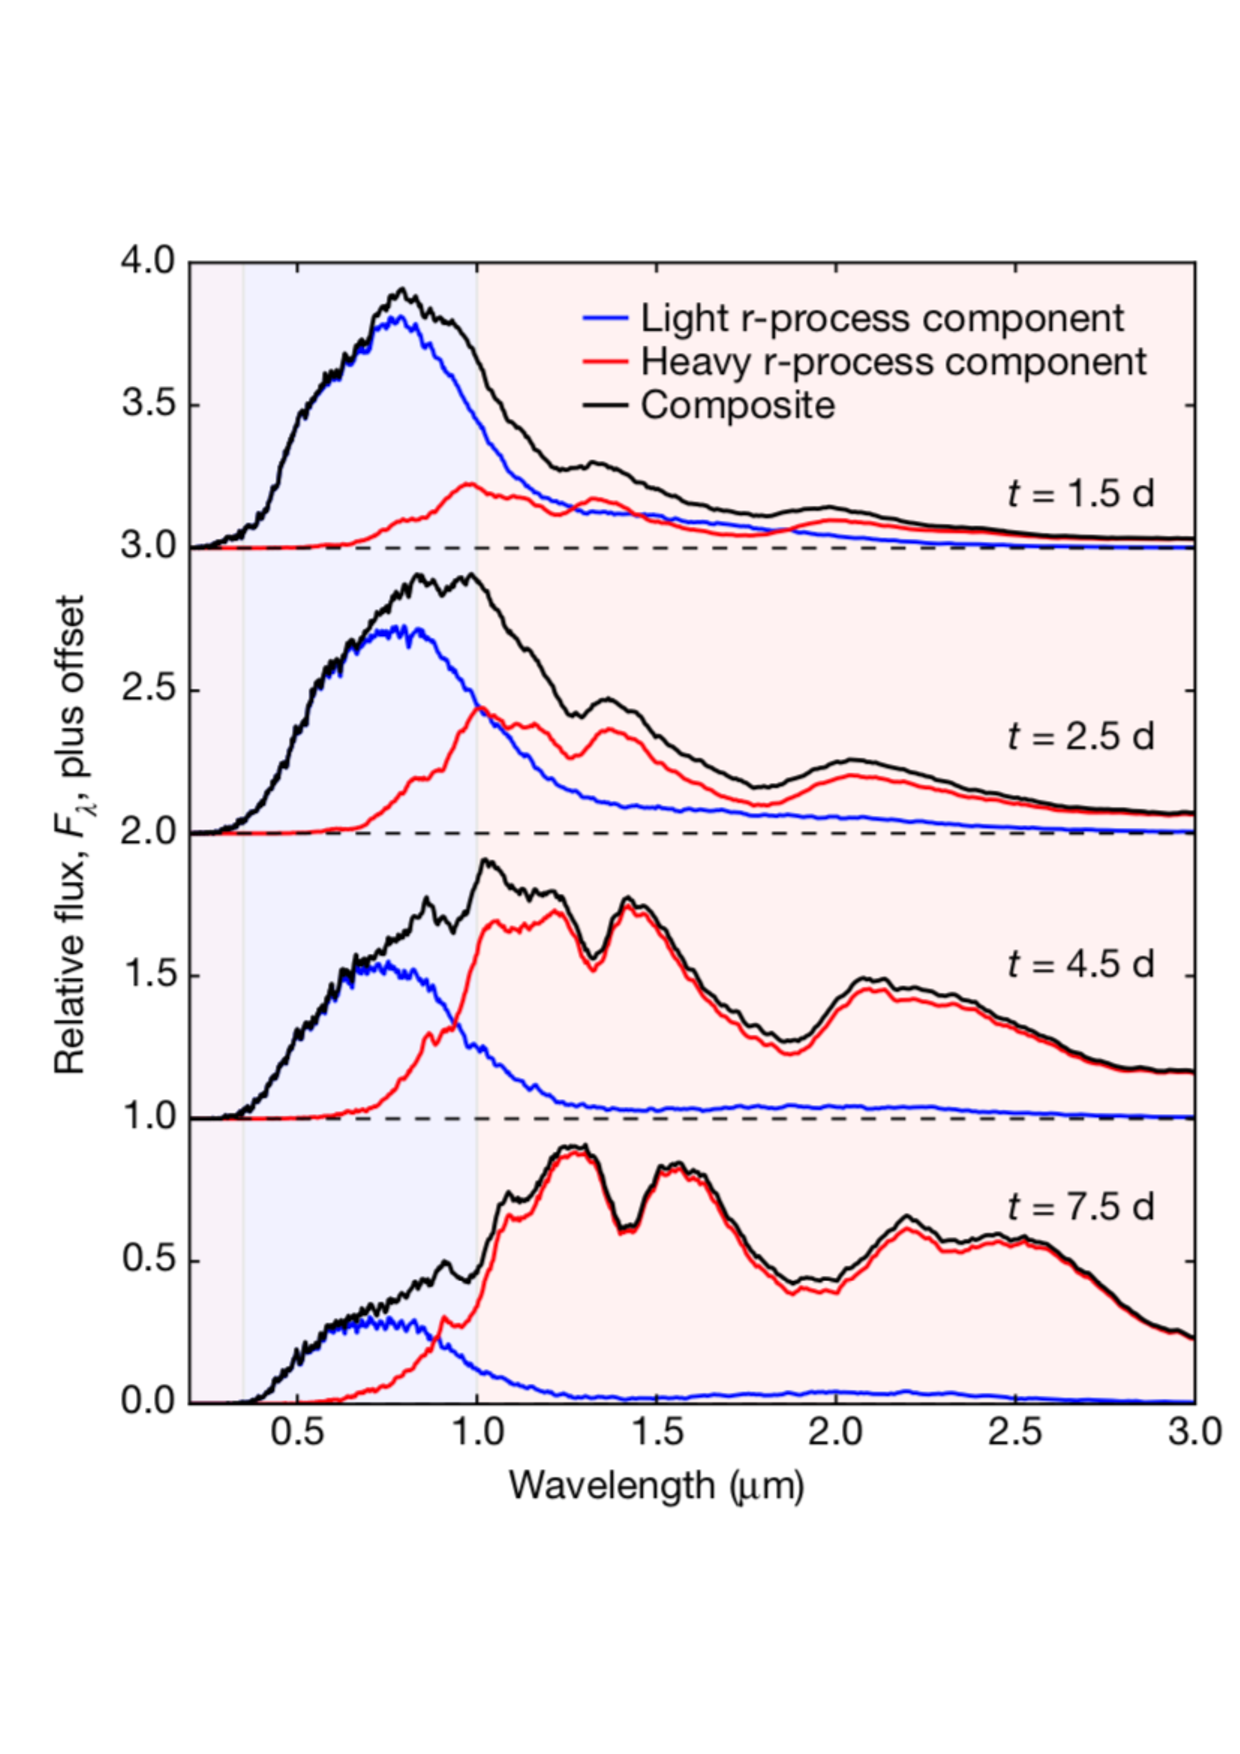
\includegraphics[width=\columnwidth]{kasen_kn} \label{kasen}
\captionof{figure}{Syntetiske spektra af en kilonova. De forskellige paneler viser tidsudviklingen, hvor man kan se at en større del af lyset blev udsendt ved længere bølgelængder i de senere tider. Dette er fordi de tungste grundstoffer forholdsvis absorberer det blå lys. Denne figure er fra \cite{kasen}}
\end{center}

\begin{center}
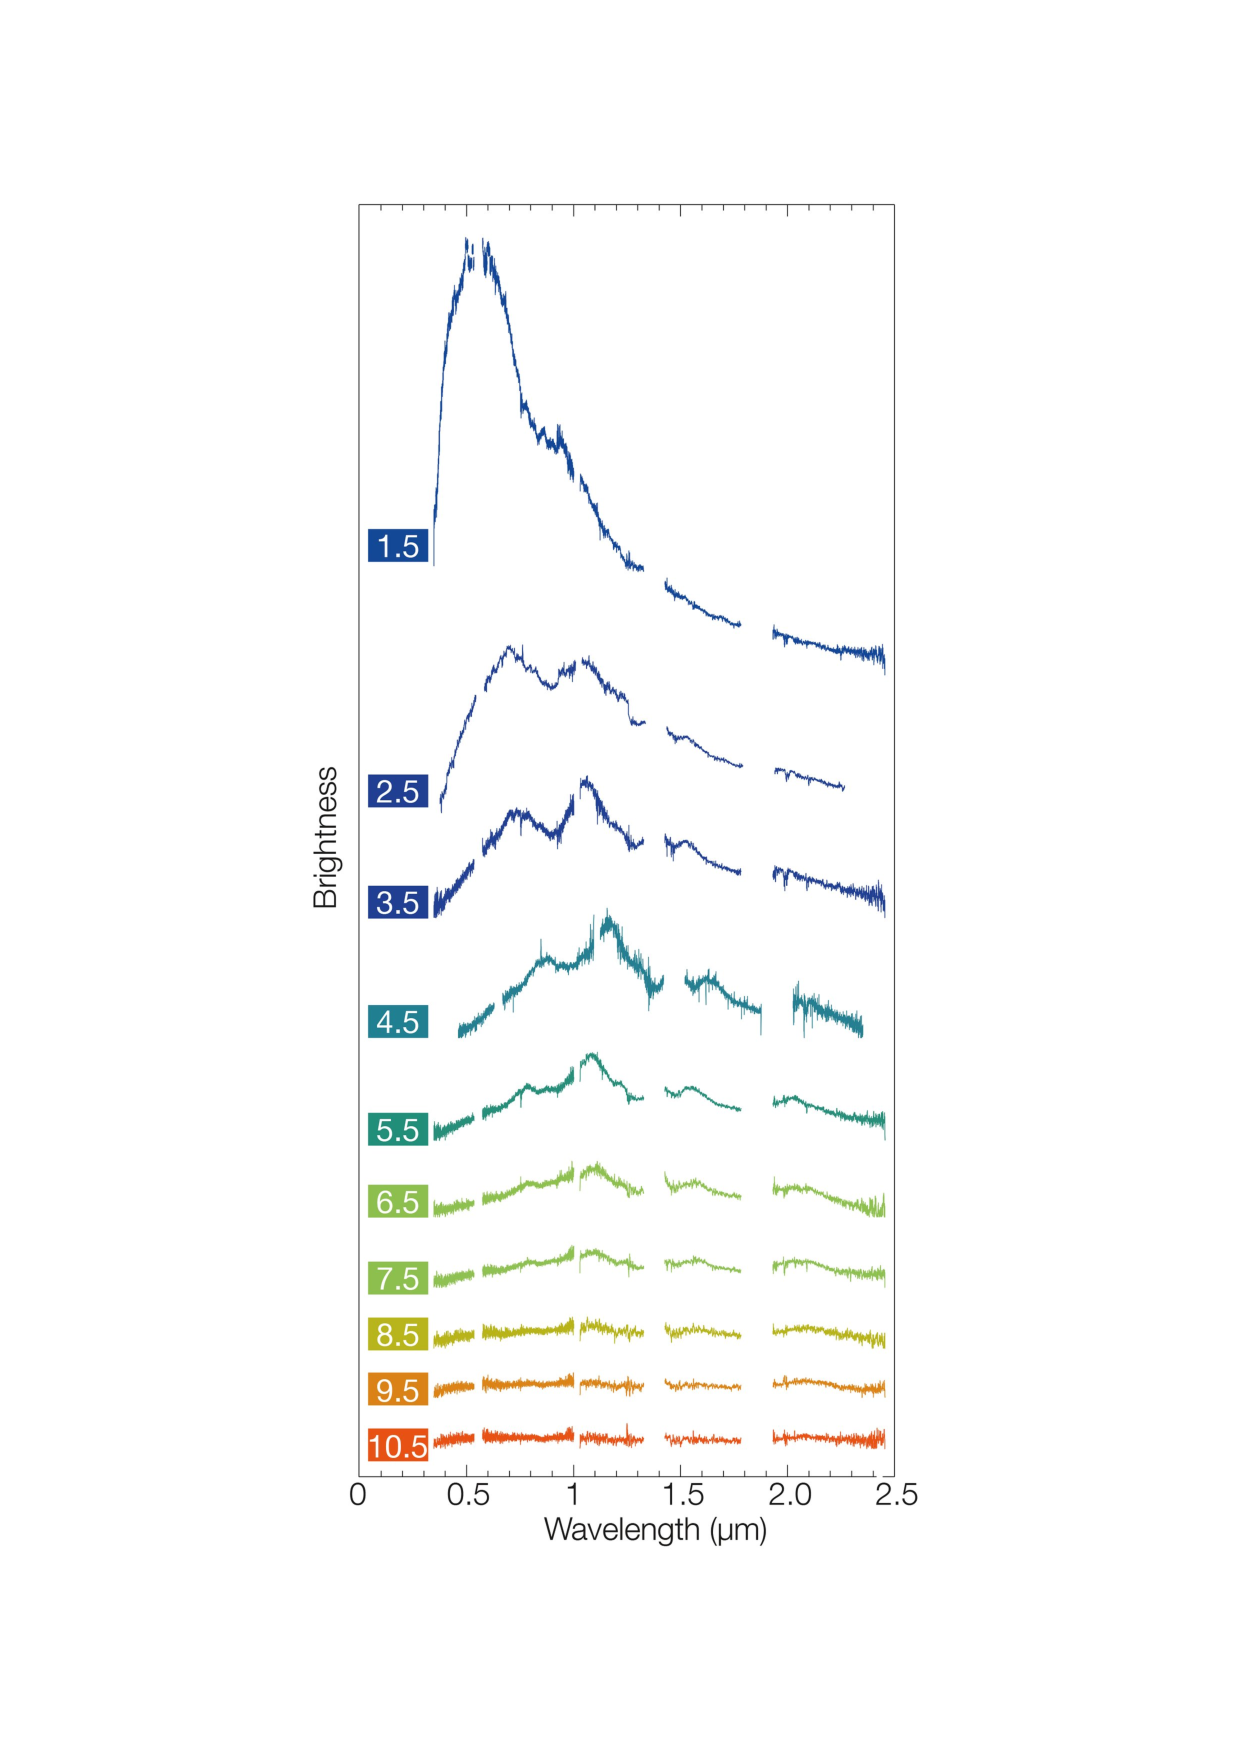
\includegraphics[width=\columnwidth]{specs.pdf}
\captionof{figure}{Spektre af kilonovaen AT2017gfo. Hvis man sammenligner spektrene med de teoretiske i figur \ref{kasen}, kan man se at den kvalitative overensstemmelse er stor. Brede signaturer, og en udvikling, hvor lyset med de korte bølgelængder forsvinder relativt til de længere. Hvad vi også kan se, er at der stadig er betydelige forskelle mellem de teoretiske of de observerede.}
\end{center}


Så, for at sammenfatte hvorfor denne detektion af tyndebøgler med et optisk modstykke er så betydningsfuld er det fordi der har med ét ført bevis for, hvad oprindelsen til korte gamma-glimt er, hvor de fleste af de tungeste grundstoffer kommer fra, samt givet en helt uafhænging måling af Hubble-konstanten.


\begin{thebibliography}{9}
\bibitem[1]{abbotta} \emph{GW170817: Observation of Gravitational Waves from a Binary Neutron Star Inspiral.},
Abbott, B. P., et al., Physical Review Letters 119, 161101 (2017).

\bibitem[2]{abbottb} \emph{Multi-messenger Observations of a Binary Neutron Star Merger.},
Abbott, B. P., et al., The Astrophysical Journal Letters, 848:L12 (2017).

\bibitem[3]{lattimer} \emph{Black-hole-neutron-star collisions.},
Lattimer, J. M. \& Schramm, D. N., The Astrophysical Journal Letters 192:L145 (1974).

\bibitem[4]{berger} \emph{Short-Duration Gamma-Ray Bursts.},
Berger, E., Annu. Rev. Astron. Astrophys. 52:43–105 (2014).

\bibitem[5]{kasen} \emph{Origin of the heavy elements in binary neutron-star
mergers from a gravitational-wave event.},
Kasen, D, et al., Nature, Volume 551, Issue 7678, pp. 80-84 (2017)

\end{thebibliography}

\begin{center}
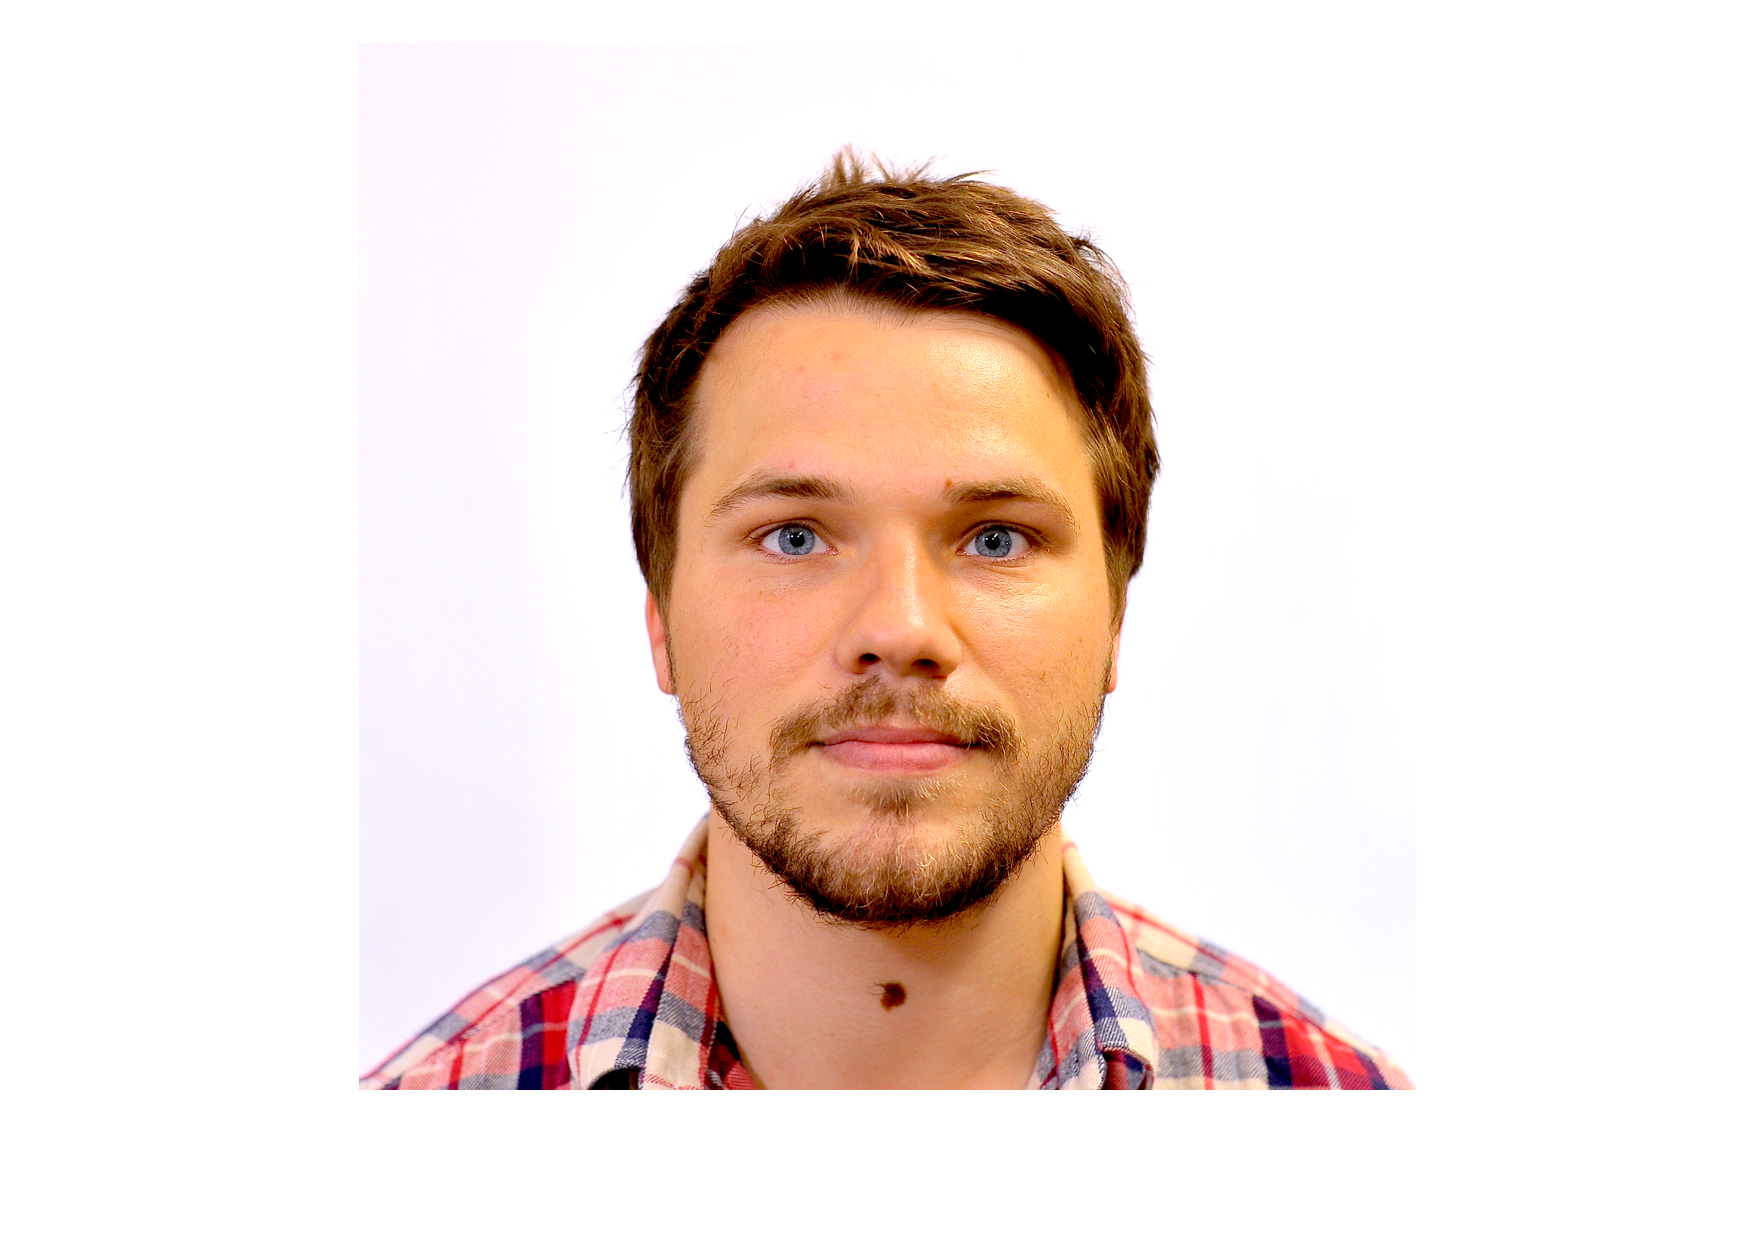
\includegraphics[width=\columnwidth]{me.pdf}
\captionof{figure}{Jonatan Selsing er postdoktoral forsker på The Cosmic Dawn Center, Niels Bohr Instituttet, Københavns Universitet.}
\end{center}

\end{document}
